\documentclass[12pt, letterpaper]{article}
\usepackage{fullpage}
\usepackage[top=1cm, bottom=4cm, left=2cm, right=2cm]{geometry}
\usepackage{amsmath,amsthm,amsfonts,amssymb,amscd}
\usepackage{lastpage}
\usepackage{enumerate}
\usepackage{fancyhdr}
\usepackage{mathrsfs}
\usepackage{graphicx}
%% download this package and put it in the same directory as this file
\setlength{\parindent}{0.0in}
\setlength{\parskip}{0.2cm}
\graphicspath{ {../figures/} }
\usepackage{subfigure}
\usepackage{float}
\usepackage{multicol}
\usepackage{multirow}
\usepackage{enumitem}
% Edit these as appropriate
\newcommand\course{DATA1030}
\newcommand\semester{Fall 2020}
\newcommand\Name{Ben Xiong}           % <-- Fill in your name here
\usepackage{lettrine}
\pagestyle{fancyplain}
\headheight 35pt
\fancyfoot{}
\lhead{\Name}
\rhead{\course\;--\;\semester}
\lfoot{}
\cfoot{}
\rfoot{\small\thepage}
\headsep 1.5em



\begin{document}

\begin{center}

	\vspace*{0.3cm}
	
	\textbf{\Large Final Report}
	
	\vspace{0.5cm}
	
	Ben Xiong
	
	DATA1030
	
	%% \vspace{0.1cm}
	
	\setlength{\parskip}{0.0in}
	
	\begin{flushleft}
	\hrulefill
	\setlength{\parskip}{0.1in}
	
	\begin{small}
	
	\textbf{Abstract:}
	This project aims to predict the average score one player can achieve against another in the game of chess. The ratings system that FIDE uses nowadays, the ELO rating, has been developed a long time ago. It is the goal of this project to find a method that has a potential boost in prediction performance in comparison to FIDE ratings.
	\setlength{\parskip}{0.0in}
	
	\hrulefill
	
	\end{small}
	
	\end{flushleft}
	
	%% \vspace{0.1cm}
	
	
	
\end{center}

\setlength{\parskip}{0.1cm}

\begin{multicols}{2}
\raggedcolumns
\subsection*{Introduction}

My project concerns some problems that are related to the game of chess. There are two main parts to my project. The first and main goal is to come up with a model that can predict the results of a chess game, while the second is to reverse-engineer some details of the current mainstream prediction system, the ELO rating system.
Although the results of a chess game can only take three discrete values (1-0, 0.5-0.5, 0-1), this is not a classification problem, since a single game between even-matched players is anyone’s match to take. We aim to predict the average score a player will obtain against another player; therefore, the validation and testing datasets must contain a sufficient number of points.

The ELO system that most nations currently use generates a score for every individual based on his/her strength that changes and becomes more accurate with the more games the play, and generally it will be possible to predict the result of a game between two players with stable ELO ratings. However, upsets happen all the time in the chess world, and it would be fun to find whether there is a better model for this problem.

I have obtained two datasets from Kaggle to work with. The first and main dataset contains the results of over 1.8 million chess games (datapoints) played amongst over 54,000 players, spread out on a 132 months period. It contains seven columns: ID of the game, month the game was played, ID of the white and black players, the outcome, and the number of games that both players played in the dataset. There is another supplementary dataset that contains the ELO ratings for around 18,000 of the players in the dataset just before everything started. This dataset was originally used in a competition that had exactly this goal, however I did not find any discussions of the specific models being used, their metrics, or their results.

The second dataset consists of just over 20,000 games played on LiChess, one of the larger online chess sites today. This dataset contains the time the games took place, the victor, number of turns, time control, some details of the opening used, and the ratings of both players. This second dataset will be used mainly for EDA, and discovering some interesting effects amongst less-experienced players.

\subsection*{EDA}

There are no missing values in either dataset. 

Using the table of initial rankings, we obtain a distribution of ~18000 players in the pool$^{[1]}$, which accounts for around one third of the total population. Even the weakest player in this pool has a rating of 2001, which roughly translates to a very strong player who can beat almost everyone who plays chess casually. The highest rated player has a rating of 2810, which would rank top ten amongst highest ratings ever achieved by humans. From these findings, we can assume that all games in this dataset are high level games.




The second dataset is much less so, being records of games by users on LiChess, most of its players are around the level of an average player who plays chess occasionally as a hobby.

White moves first in chess, and it is usually understood that white has a somewhat significant advantage in top games. We show that this is true in our main dataset.$^{[2]}$ Of all games played, the chances that white would win is almost 25\% more likely than the chances that black would win.

True to our intuition, the more frequent a player plays the game, the more likely he/she is going to win. We demonstrate this by showing two graphs of white winning chances amongst games with differently experienced players from both sides of the board.$^{3]}$

\setlength{\parskip}{0.0cm}
\begin{center}
\begin{small}
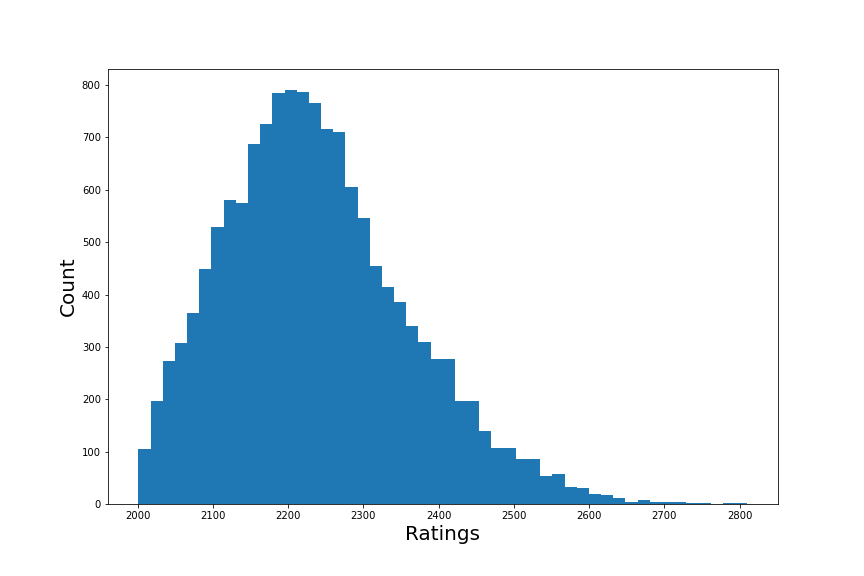
\includegraphics[width=\linewidth]{../figures/LiChessFigs/ratings_hist.png}
\textit{[1] The rating distribution in our main dataset. This dataset consists of very high-level gameplay.}
\end{small}
\end{center}

\setlength{\parskip}{0.0cm}
\begin{center}
\begin{small}
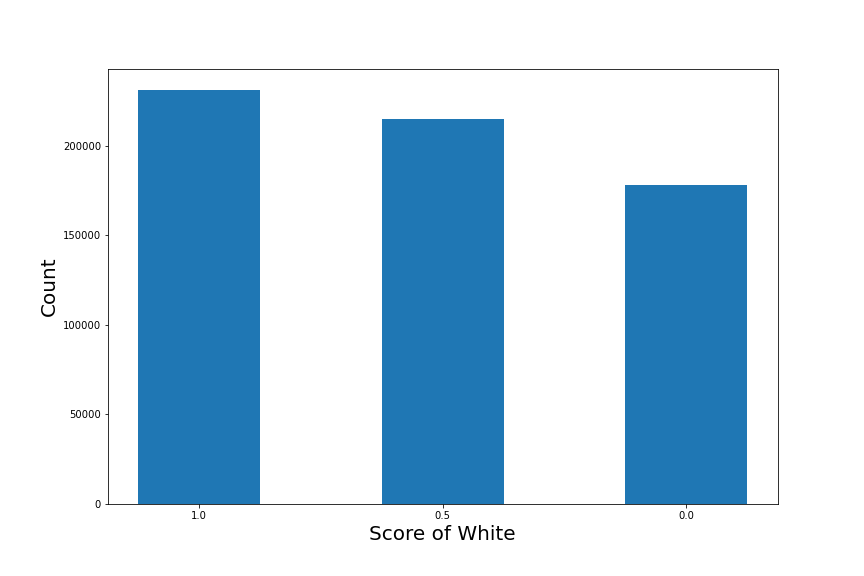
\includegraphics[width=\linewidth]{../figures/LiChessFigs/white_win.png}
\textit{[2] White wins a noticeable larger percentage of games than black. Given the amount of draws in chess, this is not as significant in the population.}
\end{small}
\end{center}

\setlength{\parskip}{0.0cm}
\begin{center}
\begin{small}
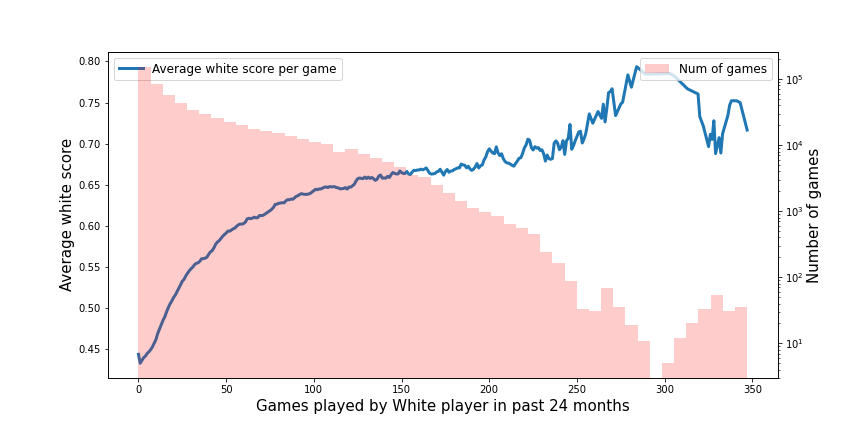
\includegraphics[width=\linewidth]{../figures/LiChessFigs/white_pre.png}
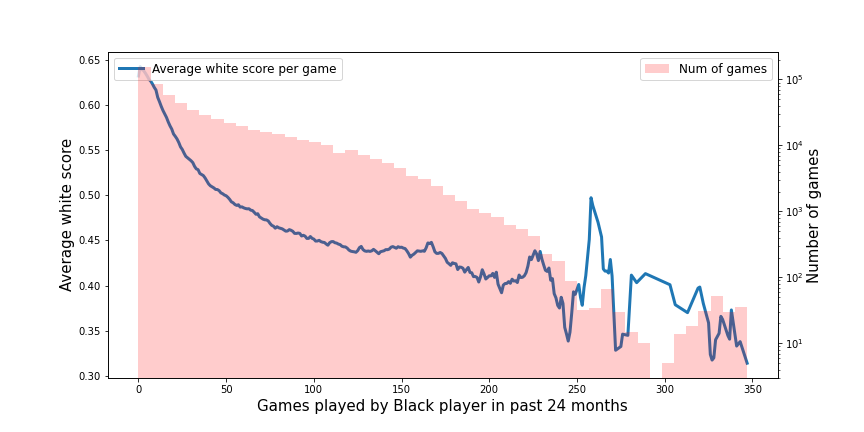
\includegraphics[width=\linewidth]{../figures/LiChessFigs/black_pre.png}
\textit{[3] The average score the white player earns per game rises with the experience of the white player, and drops with the experience of the black player.
}
\end{small}
\end{center}
\setlength{\parskip}{0.1cm}


The second dataset is mainly used for some simple experiments and fact-extraction. Because the first dataset contains a unique encoding from player to ID that does not exist in the second dataset, my model construction will be completed only on the first dataset.

It is a good idea to replace all scores with the average score the first player achieved with the second, since it’s not very reasonable to punish the model for natural discrepancies within the player’s gameplay and the factor of luck. To reiterate a point being made previously, I will aim to predict the chance that the white player will win, which is the average score the white player achieved over the black player. This will be done with data grouped on a yearly basis.

\setlength{\parskip}{0.0cm}
\begin{center}
\begin{small}
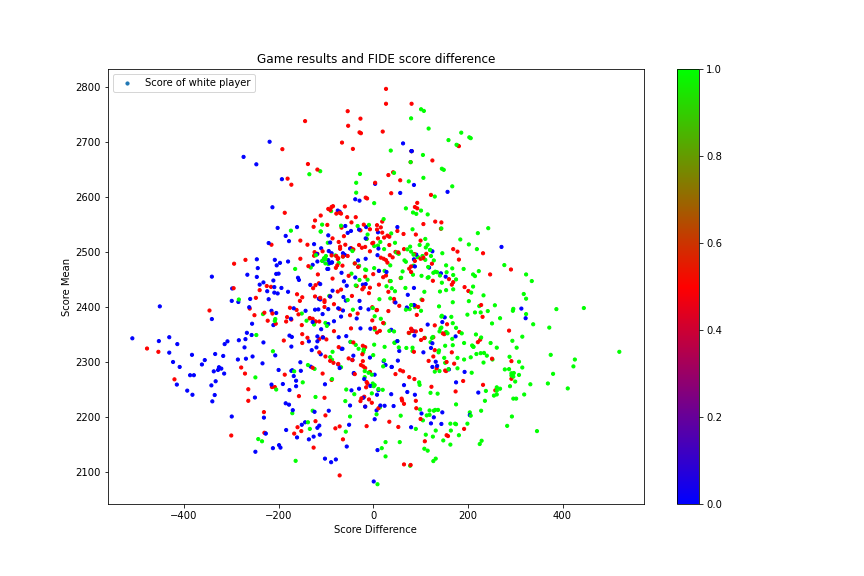
\includegraphics[width=\linewidth]{../figures/FIDE_results.png}
\textit{A plot of rating differences vs rating mean, with color code being game results. The FIDE ratings does not provide a clear distinction between games.}
\end{small}
\end{center}
\setlength{\parskip}{0.1cm}

The problem with the first dataset is that it contains far too less features for a serious prediction. To solve this problem, we will need to build some profile columns for the players based on training data. We will need to shrink the problem to “predict results of players who have a few games in the database already”. This is in fact what the original problem on Kaggle aims at. We will now need to split the data so that the validation and testing data only contains games between players that have a rather large number of previous games in the dataset. Also, considering that this dataset is time series data and thus not iid, we will adapt the following for train-test splitting: For every period of time that we wish to predict, we use up to three years of previous data to generate features through graph-based methods and a specifically designed rating algorithm. We then apply train-valid-test split of 8:1:1 on rolling periods of three years to train, tune, and evaluate the effectiveness of the entire model. We have a total of eleven years of data, the first year cannot be used because there’s not enough previous data to generate features, that means we would have 7 rolling periods of three years in total.

\subsection*{Metric}

With the labels being average games won by the white player now, we can simply use MSE as a loss metric. 

\subsection*{Models}

We will use linear regression with elastic net penalty, random forest regressor, and XGBoost regressor with elastic net penalty. The tuned parameters include l1\textunderscore ratio and alpha for all penalties, and n\textunderscore estimators and max\textunderscore depth for ensemble tree methods. SVM does not make much sense because the size of the dataset is too large, and because there is not much reason to expect that it will be better than linear models, as the data does not demonstrate locality or structure that may be suitable for a certain SVM kernel.

\subsection*{Pipeline}

To conclude everything above, the entire ML pipeline will look like the following:
\begin{enumerate}
	\item Data preprocessing, label manipulation
	\item Compute baseline model based on the first three years of games and initial rating dataset
	\item Using graphical algorithms to generate features and new rating points
	\item Create rolling periods of three years
	\item Train, valid and test on each rolling period, using all three models
	\item Find results and loss score, compare new features with baseline model
\end{enumerate}


\section*{Results}

Using the FIDE ratings of players at the starting date of the entire dataset, I built a baseline model that takes those ratings and checks to see how accurate they were in terms of predicting scores, characterized by the accuracy defined in the previous section. We can see that the predictions are basically the same, however this is because I reduced the training intensity of my model to get through the pipeline faster. I will change this in the final version of my report.

\setlength{\parskip}{0.0cm}
\begin{center}
\begin{small}
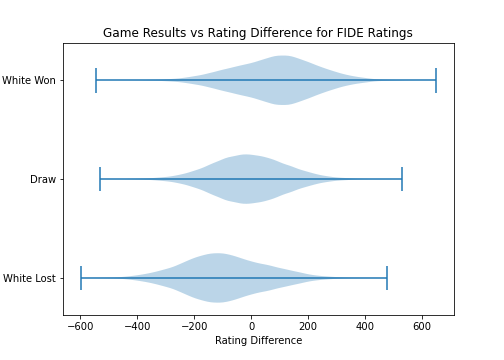
\includegraphics[width=\linewidth]{../figures/baseline_violin.png}
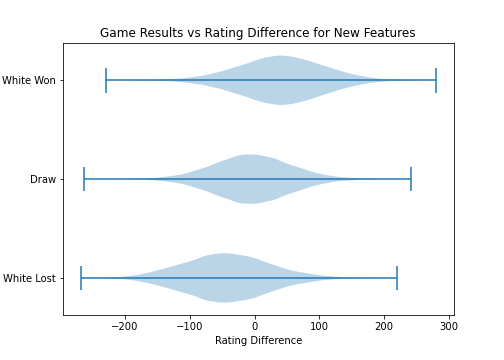
\includegraphics[width=\linewidth]{../figures/new_violin.png}
[4] These two plots demonstrate the resolution of new and old rating points. We see that the latter is not very impressive, but hopefully that will improve as I spend more time on training better models.
\end{small}
\end{center}
\setlength{\parskip}{0.1cm}

We will show several plots as comparison between our new features and the FIDE scores. This set of violin plots$^{[4]}$ demonstrates the resolution of rating difference vs the games that are won. This is a pretty simplistic and linear approach to see the effectiveness of a certain set of ratings.

Next, to even out the playing field, we will train all three models on both FIDE scores and new features. The loss will be calculated using MSE, and we demonstrate that the loss of our model is lower than its FIDE counterparts.$^{[5]}$

Feature importance and interpretations will be added here in the final version.

\setlength{\parskip}{0.0cm}
\begin{center}
\begin{small}
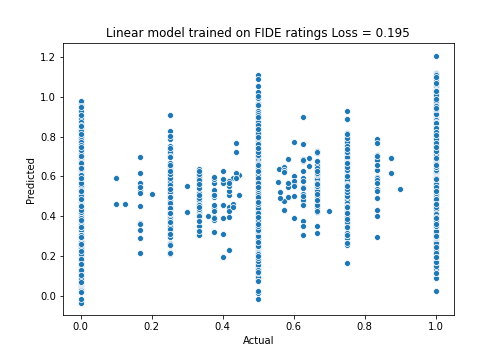
\includegraphics[width=\linewidth]{../figures/baseline_linear.png}
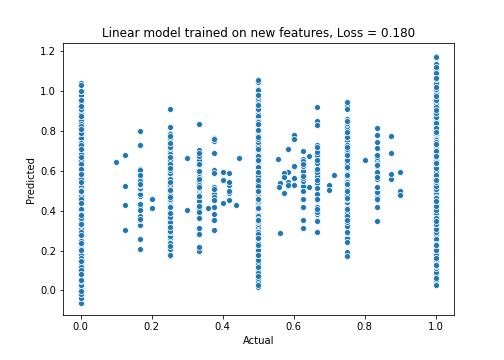
\includegraphics[width=\linewidth]{../figures/new_linear_iter_0.png}
[5] These two plots are linear models fit on the new and old features. We can see that even with a minimal amount of training, the results are already comparable.
\end{small}
\end{center}
\setlength{\parskip}{0.1cm}

\section*{Outlook}

This model has two major spaces for improvement. The first is that this model does not differentiate between the player holding white or black. This choice is made for two reasons: 

\begin{itemize}
\item splitting between the two would include halving the amount of data for each side. The data is not ample as is, and splitting it would have negative impacts on the final results.
\item The discrepancy of white wins vs black wins is not noticable enough to justify splitting the original dataset, it does not promise a significant improvement in performance.
\end{itemize}

With that said, this is still a direction to go with more data in hand. However with chess games being somewhat hard to collect, especially high-level games, this might not be such a promising direction. (It’s worth mentioning that recently chess.com has seen surges in their user’s games, this includes many matches between top grandmasters in the world. However it is also widely accepted that online chess does variate from OTB, or “over the board” chess by a lot.)
Secondly, this model does not fully account for “loops”, or rock-paper-scissor cycles between player’s playing styles. In fact, when creating the graphical model to generate ratings, even as the player’s ratings are stationary there still exists some large points transfers within every iteration. To translate, this means an observable part of wins are not purely predictable by the ratings generated.


\section*{References}
\begin{small}
\begin{flushleft}
	\textit{Deloitte/FIDE Chess Ratings Challenge, Kaggle,}
	\textit{https://www.kaggle.com/c/ChessRatings2/data}
	
	\textit{Chess Game Dataset (LiChess), Kaggle,} 
	\textit{https://www.kaggle.com/datasnaek/chess}
\end{flushleft}
\end{small}


\section*{Github Repo}
	\textit{https://github.com/PolarBearXBK/1030Chess}
\end{multicols}	

%\begin{figure}[H]
%    \centering
%    % replace "dim.png" with your image file, placed in the same directory
%    \includegraphics[width=0.6\linewidth]{Results.png}
%    % give it a name
%    \caption{My Plot}
%\end{figure}

\end{document}